\subsection{Datenbeschaffung}
\label{subsec:Datenbeschaffung}
Durch die verschiedenen Property Management Systeme sind für die einzelnen Hotels bereits Stammdaten wie Zimmeranzahl oder Zimmerkategorien vorhanden. Zudem wird der jeweilige Kunde beim Einrichten von happyhotel auch schon nach verschiedenen Daten befragt. Unter den Daten, die bei einem Kunden abgefragt werden, gehören Informationen wie zum Beispiel die Adresse des jeweiligen Hotels. 
\newline
\newline
Werden nun alle schon vorhanden Informationen zusammengetragen, die bisher in der Datenbank zur Verfügung stehen, entsteht dabei das folgende Dataframe:
\begin{figure}[h]
    \centering
    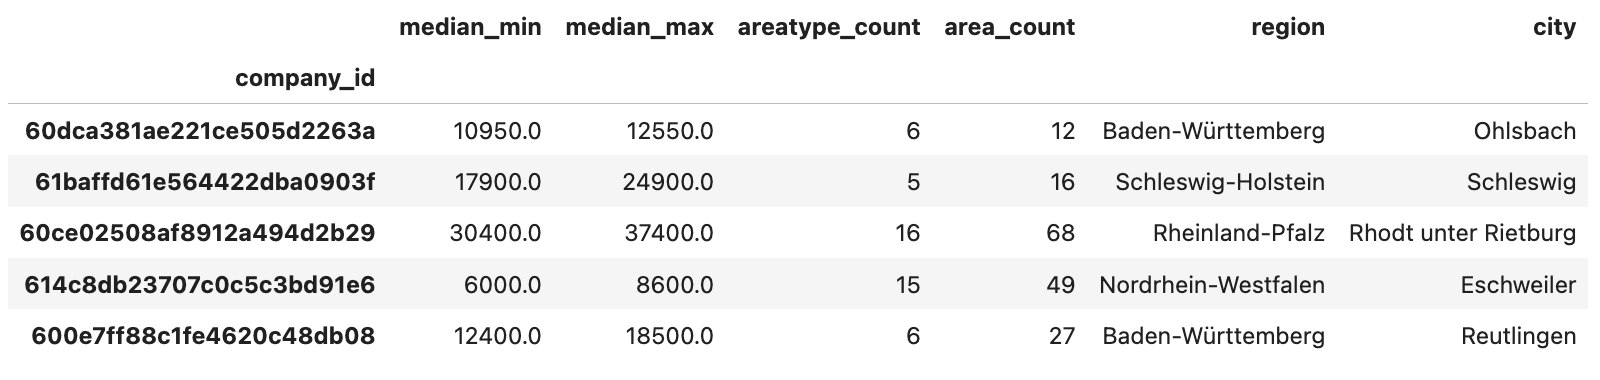
\includegraphics[width=1\textwidth, center]{Features_1.png}
    \caption[Alle schon vorhanden Features]{Alle schon vorhanden Features}
    \label{img:all_Features}
\end{figure}

In Abbildung \ref{img:all_Features} sind die Daten zu sehen, die bislang zur Verfügung stehen, wobei sich die \emph{median\_min} und \emph{median\_max} Werte auf den Median aller Zimmerkategorie-Preise bezieht.
\newline
\newline
Dadurch, dass \emph{region} und \emph{city} manuell vom Kunden eingetragene Werte sind, ergab sich eine gewisse Skepsis, ob alle Werte norm-konform eingetragen wurden. Aufgrund dieser Skepsis sollte eine kleine Datenanalyse getätigt werden. 
\newline
\newline
Bei der Datenanalyse wurde jeweils nach der Region und nach der Stadt gruppiert, um zu prüfen ob die Daten so benutzt werden können. Im Folgenden sind die Werte jeweils für die Region und für die Stadt zu sehen:

\begin{figure}[h]
    \centering
    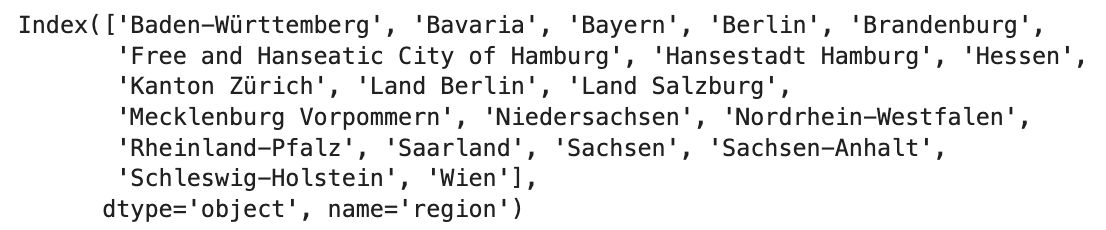
\includegraphics[width=0.8\textwidth, center]{region_1.png}
    \caption[Alle vorhanden Regionen]{Alle vorhanden Regionen}
    \label{img:region_1}
\end{figure}

\begin{figure}[h]
    \centering
    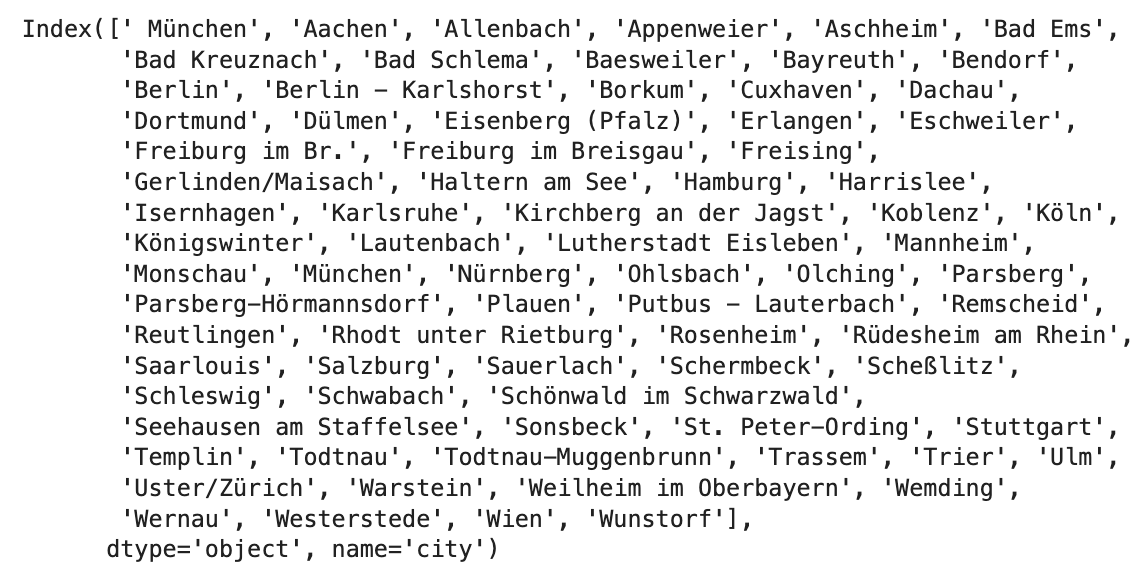
\includegraphics[width=0.8\textwidth, center]{city_1.png}
    \caption[Alle vorhanden Städte]{Alle vorhanden Städte}
    \label{img:city_1}
\end{figure}

Es ist eindeutig zu erkennen, dass es sowohl bei der Region als auch bei der Stadt zu einer Inkonsistenz kommt. So wurde die Region \emph{Berlin} sowohl als \emph{Berlin}, als auch mit \emph{Land Berlin} angegeben. Auch bei der Stadt ist die Diskrepanz deutlich zu erkennen, -so wurde bspw. \emph{München} mit Leerzeichen vorne dran angegeben oder die Stadt Freiburg einmal mit der Abkürzung \emph{Br.} und ein anderes Mal mit komplett ausgeschriebenen \emph{Breisgau} angegeben. Es ergab sich also, dass diese Werte so wie sie sind, nicht verwendet werden können.

\subsubsection{Beschaffung von Region, City und Stadtgröße}
\label{subsubsec:region_city_size}
Durch eine schon im Vorfeld getätigte Arbeit, existiert zu jedem Hotel in unserer Datenbank, die Koordinaten, repräsentiert durch die zwei Werte Long- und Latitude. Mithilfe von diesen zwei Werten sollte ein Skript geschrieben werden um die Region, die Stadt und Größe der Stadt zu beschaffen. 
\newline
\newline
Für das Skript wurde \emph{Nominatim} API verwendet um die einzelnen Werte zu beschaffen. Im folgenden wird das Skript präsentiert:

\begin{lstlisting}[language=Python, label=lst:RS_Demo, caption=Einfaches Recommendation System für Film vorschläge]
    from geopy.geocoders import Nominatim

def get_region_city_size(latitude, longitude):
    geolocator = Nominatim(user_agent="city_size_app")
    location = geolocator.reverse((latitude, longitude), language='de')

    address = location.raw['address']

    if 'city' in address:
      region = address["city"]
      if 'state' in address:
        region = address["state"]
      return {
            "city": address["city"],
            "region": region,
            "size": "Großstadt"
        }
    elif 'town' in address:
        return {
            "city": address["town"],
            "region": address["state"],
            "size": "Kleinstadt"
        }
    elif 'village' in address:
      region = None
      if 'county' in address:
        region = address["county"]
      if 'state' in address:
        region = address["state"]
      return {
            "city": address["village"],
            "region": region,
            "size": "Kleinstadt"
        }
    else:
        return dict()
\end{lstlisting}

Die Funktion \emph{get\_region\_city\_size} nimmt als Parameter die Long- und Latitude Werte und erzeugt dadurch ein \emph{Dictionary} mit den Werten \emph{region}, \emph{city} und \emph{size}.
\subsubsection{Beschaffung von der Hotelart}
\label{subsubsec:hotelart}
Einer der wichtigsten Eigenschaften, die ein Hotel vorweisen kann, ist die Hotelart von dem jeweiligen Hotel. Die Hotelart hängt maßgeblich mit der zur grundlegenden Preisgestaltung ab. Dies ist einfach zu erklären, da Hotels existieren, die eher auf Wellness ausgelegt sind und somit prinzipiell teurer sind als einfache Urlaubshotels. Somit ist die Art eines Hotels essentiell um ähnliche Hotels zu finden. So soll auch für das Modell die Hotelart vorhanden sein. Dieses Feature muss jedoch erst beschafft werden, da diese Information nicht in der Datenbank hinterlegt ist. 
\newline
\newline
Leider ist der Versuch, die Hotelart auf einem automatisiertem Weg zu bekommen, gescheitert und es blieb nichts anderes übrig als die Hotelart eines jedem Hotels manuell herauszufinden. 
\newline
\newline
Nachdem die Hotelart beschaffen wurde, sieht der Feature-Datensatz wie folgt aus:
\begin{figure}[h]
    \centering
    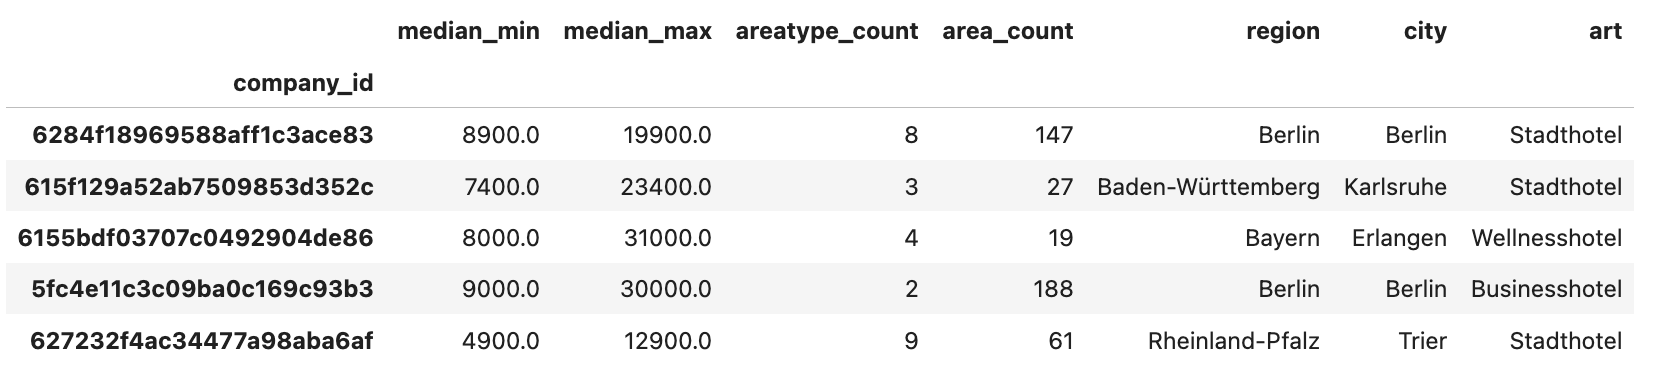
\includegraphics[width=1\textwidth, center]{Features_2.png}
    \caption[Alle schon vorhanden Features #2]{Alle schon vorhanden Features #2}
    \label{img:all_Features_2}
\end{figure}
